% !TEX TS-program = pdflatexmk
\documentclass[12pt]{article}
 \usepackage[margin=1in]{geometry} 
\usepackage{amsmath,amsthm,amssymb,amsfonts}
 \newtheorem{definition}{Definition}[section]
 \newtheorem{theorem}{Theorem}[section]
  \newtheorem{sats}{Sats}[section]
\usepackage[most]{tcolorbox}
\setlength{\parindent}{0.0in}
\setlength{\parskip}{0.05in}
\usepackage{empheq}
\usepackage{float}

\usepackage{framed}
\usepackage[most]{tcolorbox}
\usepackage{xcolor}
\colorlet{shadecolor}{orange!15}
\parindent 0in
\parskip 12pt
\geometry{margin=1in, headsep=0.25in}
\usepackage{amsthm}
\usepackage[utf8x]{inputenc}
\usepackage{comment}
\usepackage{xcolor}
\newcommand{\N}{\mathbb{N}}
\newcommand{\Z}{\mathbb{Z}}
\usepackage{graphicx}
\usepackage{pgf,tikz,pgfplots}
\pgfplotsset{compat=1.15}
\usepackage{mathrsfs}
\usetikzlibrary{arrows}
\usepackage{subcaption}
\pagestyle{empty}
\usepackage{systeme}
\usepackage{pgfplots}
\usepackage{hyperref}
\usepackage{amsthm} 
\newenvironment{solution}
  {\renewcommand\qedsymbol{$\blacksquare$}\begin{proof}[Solution]}
  {\end{proof}}
 
\usepackage[]{algorithm2e}

\newenvironment{problem}[2][Problem]{\begin{trivlist}
\item[\hskip \labelsep {\bfseries #1}\hskip \labelsep {\bfseries #2.}]}{\end{trivlist}}
%If you want to title your bold things something different just make another thing exactly like this but replace "problem" with the name of the thing you want, like theorem or lemma or whatever
\usepackage{mathtools}

%TO HIGHLIGHT USE \hl
\usepackage{xcolor}
\usepackage{soul}
\usepackage{bm}

\usepackage{epigraph}


\usepackage{dirtytalk}

\usepackage{mathtools}
\DeclarePairedDelimiter{\innerprod}\langle\rangle
\newcommand\conjinnerp[2][]{\:\overline{\mkern-4mu\innerprod[#1]{#2}\mkern-4mu}\:}
\usepackage{fancyhdr}
\pagestyle{fancy}
\fancyhf{}
\rhead{Machine Learning}
\lhead{Kiar Fatah}
\rfoot{Page \thepage}


\numberwithin{equation}{section}

\title{Machine Learning}

\author{Kiar Fatah}

\date{\today}
\begin{document}

\maketitle

\newpage

\tableofcontents 

\newpage
\epigraph{If you can’t explain something in simple terms, you don’t understand it.}{\textit{Richard Feynman }}
\newpage

\section{Lecture 2}
\subsection{Decision Tree}
A decision tree is a map of the possible outcomes of a series of related choices.
\subsection{How to build a Tree}
\begin{enumerate}
\item Choose the best question (according to the information
gain), and split the input data into subsets.
\item Terminate: call branches with a unique class labels leaves
(no need for further questions).
\item Grow: recursively extend other branches (with subsets bearing mixtures of labels).
\end{enumerate}

\subsection{How to ask the best questions?}
The machine will automate the questions for the decision tree, however how does it obtain the best questions to ask? It does so by with the help of Gini impurity and information gain.
\subsubsection{Gini impurity}
Gini impurity is a measurement of uncertainty in a node. It is calculated by how often a randomly chosen element from the set would be incorrectly labeled if it was randomly labeled according to the distribution of labels in the subset. 
\begin{equation}
    1 - \sum_i p_i^2.
\end{equation}
\subsubsection{Entropy}
Entropy is also a measurement of uncertainty in a node and can be applied instead of Gini impurity. It is calculated as
\begin{equation}
    \sum_i -p_ilog_2 p_i.
\end{equation}
The information entropy is measured in bits, corresponding to the logarithmic base 2. Tossing a coin results in the entropy 1, hence it has 1 bit of information. For a real dice and a fake dice the value is 2.58 and 2.16 bits of information respectively.

\subsubsection{Information gain}
Information gain is how much the question reduces the uncertainty. The information is given by the first set of values for the internal node subtracted by the average value of the impurity of the split set. 

\subsubsection{Best question}
The question with the \hl{highest value} on the information gain will be the one to ask.

\subsection{Overfitting}
Overfitting is when the learned models are overly specialised for the training samples. This occurs when the data is too noisy, not representative and when the model is too complex. This can be tackled by choosing a simpler model.

\subsubsection{Pruning}
The idea of reduced error pruning is to consider each node in the tree as a candidate for removal. A node is removed if the resulting pruned tree performs at least as well as the original tree over a separate validation dataset. The pruning is done on validation set, until it is harmful for the model.

\subsubsection{Validation set}
Due to pruning there is a need for validation dataset that is not training nor test data set. Therefore if there is access to a rich data set, it is separated to three categories. In essence the validation set is used to estimate prediction error for model selection (i.e. to determine hyperparameters).

\section{Lecture 3}

\subsection{Introduction}
How does one determine the right model, f, from the data? The simple concept for classification is by calculating the misclassification rate in consideration to the data. Assume the following data is given $\mathcal{D} = {(\bm{x_1},y),....}$ is given. The misclassification rate is given by
\begin{equation}
err(f,\mathcal{D}) = \frac{1}{N}\sum Ind(f(\bm{x}) \neq y)
\end{equation}

\subsection{Curse of Dimensionality}
\begin{enumerate}
    \item Easy problems in low-dimensions are harder in high-dimensions, e.g training more complex models with limited sample data.
    \item In high-dimensions everything is far from everything else, this is an issue in the nearest neighbour model, this causes issues with Nearest Neighbours.
    \item Any method that attempts to produce locally varying functions in small isotropic neighbourhoods will run into problems in high dimensions.
\end{enumerate}


\subsection{The Bias-Variance Trade-off}
Let us imagine we could repeat the modelling for many times – each time by gathering new set of training samples, D. The resulting models will have a range of predictions due to randomness in the underlying data set.
\begin{enumerate}
    \item Variance: Refers to the amount by which $\hat{f}$, the prediction function, would change if we estimated it using a different training data set.
    \item Bias: Refers to the error that is introduced by approximating a real-life problem, which may be extremely complicated, by a much simpler model.
\end{enumerate}
This can be showcased in figure \ref{var_bias}
\begin{figure}[!ht]
    \centering
    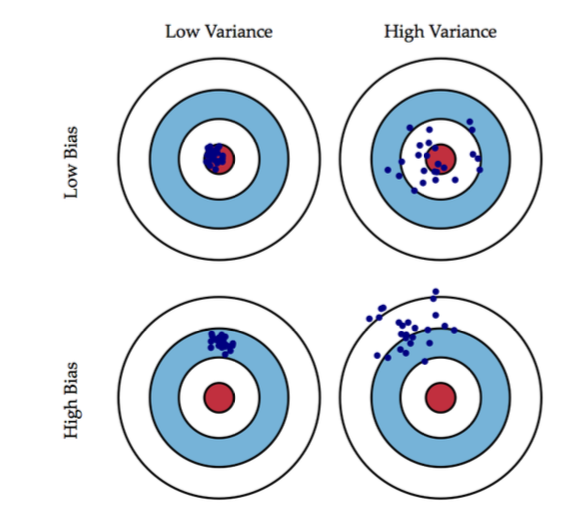
\includegraphics[scale = 0.7]{var_bias.png}
    \caption{Variance versus Bias}
    \label{var_bias}
\end{figure}
In essence the relationship between complexity, bias and variance can be summarised as
\begin{enumerate}
    \item Low model complexity implies high bias, low variance.
    \item High model complexity implies low bias, high variance.
\end{enumerate}
Note that bias and variance are equally important as we are always dealing with a single realisation of the data set.

\section{Lecture 4}

\subsection{Linear Regression, A Parametric Method}
Simple linear regression assumes theres a linear relationship between the output and input. Therefore a linear equation is assumed, parametric method. However, the coefficients are unknown and thus needs to be approximated. 

The measurement of error is mean square. It is a convex function. Therefore the coefficients that minimises the sum of the squared error is given by the vector that sets the gradient of the sum of squared error to zero.

\begin{equation}
E_{in} (w) = ||Xw - Y ||^2 \implies \frac{\partial E_{in}}{\partial w} =  2X^T(Xw - Y) = 0 \implies w = (X^T X )^{-1}X^T Y
\end{equation}
whereas w is the coefficients, X the data, Y the label and $E_{in}$ the sum of squared errors.

\subsection{RANdom SAmpling Consensus}
Random sampling consensus or RANSAC is applied when the data set S contains outliers
\begin{enumerate}
    \item Randomly select a (minimum number of) sample of s data
    points from S and instantiate the model from this subset.
    \item Determine the set of data points $S_i$ which are within a distance threshold t of the model. The set $S_i$ is the consensus set of samples and defines the inliers of S.
    \item If the subset of $S_i$ is greater than some threshold T, re-estimate the model using all the points in Si and terminate
    \item If the size of $S_i$ is less than T, select a new subset and repeat the above.
    \item After N trials the largest consensus set $S_i$ is selected, and the model is re-estimated using all the points in the subset $S_i$
\end{enumerate}
In essence RANSAC takes two random data points and fits a line. This is repeated until there is a good result of data points within the margin of the fitted line. RANSAC is applied when the dataset contains outliners.
\begin{figure}[!ht]
    \centering
    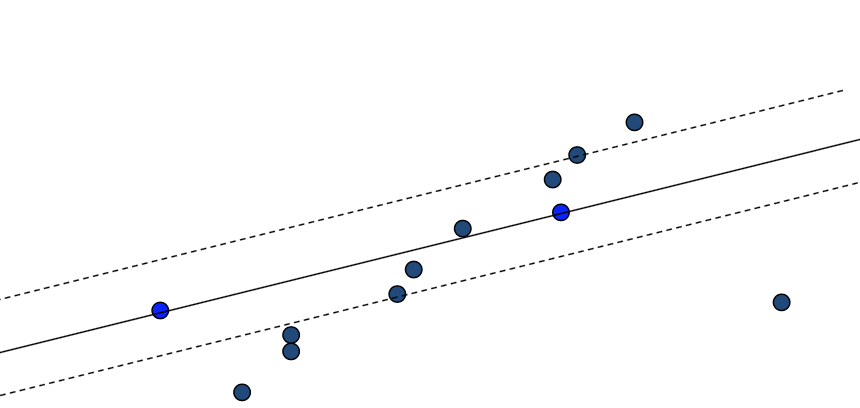
\includegraphics[width =9cm]{RANSAC.png}
    \caption{Line fitting between two data points.}
    \label{RANSAC}
\end{figure}

\subsection{Disadvantages with RANSAC}
The threshold of the margin in the line is vulnerable.
\begin{enumerate}
\item  If it is to high every fit is ranked equally. 
\item If it is to low it leads to an unstable fit.
\end{enumerate}
However, this issues are tackled within MLESAC that evaluates the quality of the consensus dataset by calculating its likelihood for better predictions.


\subsection{k-NN Regression, A Non-parametric}
The k-NN regression method is closely related to the k-NN classifier. Given a value for K and a prediction point $x_0$, k-NN regression first identiffies the K training observations that are closest to $x_0$ represented by $N_0$. It then estimates $f(x_0)$ using the average of all the training responses in $N_0$. In other words
\begin{equation}
    \hat{f(x_0)} = \frac{1}{K} \sum_{x_i \in N_0} y_i.
\end{equation}
Note larger values of k provide a smoother and less variable fit (lower variance!)

\subsection{Parametric or Non-parametric Methods?}
\begin{enumerate}
    \item  If the parametric form is close to the true form of f, the parametric approach will outperform the non-parametric
    \item As a general rule, parametric methods will tend to outperform non-parametric when there is a small number of observations per predictor (i.e. in a high dimension).
    \item Interpretability stand point: Linear regression preferred to KNN if the test MSEs are similar or slightly lower.
\end{enumerate}

\subsection{Shrinkage Methods}
A common way to fit models is by applying least square, however an alternative is it is possible to fit a model containing all p predictors using a technique that constrains or regularizes the coefficient estimates, or equivalently that shrinks the coefficient estimates towards zero.
\begin{enumerate}
    \item Among a large number of variables X in the model there are generally many that have little (or no) effect on Y
    \item Leaving these variables in the model makes it harder to see the big picture, i.e. the effect of the “important variables”
    \item Would be easier to interpret the model by removing unimportant variables (setting the coefficients to zero)
\end{enumerate}

\subsection{Ridge Regression}
Similar to least squares but minimizes different quantity
\begin{equation}
RSS + \lambda \sum_i w_i^2
\end{equation}
Note that the second term is called shrinkage penalty.
\begin{enumerate}
    \item Shrinkage penalty is a small value when the coefficients $w_i$ are close to zero.
    \item The parameter $\lambda$ controls the impact of the two terms. Hence the selection is critical.
    \item For a higher value on $\lambda$ the variance decreases and bias increases.
    \item Ridge regression is harder to interpret.
\end{enumerate}

\subsection{The Lasso}
Similar to least squares but minimizes different quantity
\begin{equation}
RSS + \lambda \sum_i |w_i|
\end{equation}

\section{Lecture 5}

\subsection{Axiomatic definition of probabilities}
Given an sample space $\omega$ of all possible outcomes, and an event E, or set of outcomes from $\omega$ then
\begin{enumerate}
    \item $P(E) \geq 0$ for all $E \subseteq \omega$.
    \item If $E = \omega$ then the probability of $\omega$ is one. In other words the probability that one event will occur is equal to one.
    \item if the events are a ocuntable sequence of pairwise disjoint events then the probability of the union of each event is equal to the probability of the summation of every event.
\end{enumerate}
\subsection{Random (Stochastic) Variables}
A random variable is neither random nor a variable, it is a function that does exactly what we need, $X: \Omega \to \mathbb{R}$.
The probability distribution function, so called pdf, of a random variable maps the range to positive numbers, $Pr(x): X \to \mathbb{R}_{>0}$.
\begin{enumerate}
    \item The probability of a random variables describes how the probability density is distributed over the range of X,
    \begin{equation}
        P[0 \leq X \leq 1] = \int_{x = 0}^1 Pr(x) dx.
    \end{equation}
    \item X is distributed Pr(x) is written ore compactly as 
    \begin{equation}
        X \sim Pr(x).
    \end{equation}
\end{enumerate}
An example is 
\begin{enumerate}
\item $\Omega$ - All possible graded exams of all students in class.
\item $X: \Omega \to \mathbb{R}$ - Random variable mapping exam outcome to score.
\item $X \sim Pr(x)$ - Gaussian distribution.
\end{enumerate}


\subsection{Types of Random Variables}
\begin{enumerate}
    \item Discrete random variable: Countable set
    \item Continuous random variable: Uncountable set
\end{enumerate}

\subsection{Joint Probabilities}
Consider two random variables X and Y. Observe multiple paired instances, some paired outcomes will occur frequently. This information is encoded in the joint probability density function $Pr(x,y)$.

\subsection{Marginalization}
The probability distribution function, PDF, of any single variable can be recovered from a joint distribution by summing for the discrete case and integrating for the continuous case.
\begin{equation}
    Pr(x) = \sum_y Pr(x,y), (Discrete)
\end{equation}

\subsection{Conditional Probabilities}
The conditional probability of X given that Y takes a value y gives
\begin{equation}
    P(A|B) = \frac{P(A, B)}{P(B)}.
\end{equation}
If it turns out the events are independent then
\begin{equation}
    P(A|B) = \frac{P(A) P(B)}{P(B)}.
\end{equation}
Bayes's theorem gives us
\begin{equation}
    P(A | B) = P(A|B)P(B) = P(B|A)P(A) \implies P(A|B) = \frac{P(B|A) P(A) }{P(B)}.
\end{equation}

\subsection{Common Distributions}
\begin{enumerate}
    \item Bernoulli - is a discrete distribution that models binary trials.
    \item Categorical - is a discrete distribution that determines the probability of observing one of k possible outcomes. Bernoulli distribution is a special case of categorical distribution.
    \item Gaussian or Univariate normal distribution - is a continuous distribution.
\end{enumerate}

\subsection{Central Limit Theorem}
The distribution of a linear combination of a large number of
independent, identically distributed (iid) variables will tend to
normal, regardless of the underlying distribution.

\subsection{Expectation}
Given a function, $f[*]$, that returns a value for each possible value $x^*$ of the variable $x$ and a probability $Pr(x = x^*)$ that each value of x occurs. The expected output of that fuction is calculated according to
\begin{equation}
    \mathbb{E}[X] = \mu_X = \int x Pr(x) dx.
\end{equation}
it is equal to the center of gravity of a distribution. However, for different choices of the function, $f[*]$, the interpretation is different. Hence the variance can be calculated as
\begin{equation}
    Var[X] = \sigma_X^2 = \mathbb{E}[X-\mathbb{E}[X])^2],
\end{equation}
and is interpreted as the spread of a distribution. The covariance is given by
\begin{equation}
    \sigma_{X,Y} = \mathbb{E}[X-\mathbb{E}[X]](Y-\mathbb{E}[Y])],
\end{equation}
it showcases how two variables vary together.
\subsection{General Machine Learning Problem}
if Y is discrete then it is classification, if it is continuous it is regression.
\begin{enumerate}
    \item Learning: We estimate Pr($\bm{x}$, y) from data.
    \item Inference: We estimate $Pr(y | \bm{X} = \bm{x}$) from data.
\end{enumerate}

\subsection{Bayes's Rule}
\begin{enumerate}
    \item $Pr(\bm{x} | Y = y)$: Likelihood represents the probability density of observing data $\bm{x}$ given the hypothesis Y = y
    \item $Pr(Y = y)$: Prior represents the knowledge about Y before any observation.
    \item $Pr(y | \bm{X} = \bm{x})$: Posterior represents the probability density of hypothesis y given observation $\bm{X} = \bm{x}$.
    \item $Pr(\bm{X} = \bm{x})$: Evidence describes how well the model fits the evidence.
\end{enumerate}

\subsection{Probabilistic Regression}
Regression via conditional probability:
\begin{enumerate}
\item Find the joint distribution of $\bm{X}$ and Y: Pr($\bm{X}$,y)
\item Compute the posterior of Y: $Pr(y| \bm{X} = x) = \frac{Pr(\bm{x},y)}{Pr(\bm{X} = x)}$
\item Compute conditional expectation: $\mathbb{E}[Y |X = x]$.
\end{enumerate}
Explicit regression model:
\begin{enumerate}
\item Define a deterministic model $y = f(\bm{x}) + \epsilon$.
\item Describe probability distribution of the error $\epsilon = y -  f(\bm{x}) $.
\item Estimate the parameters in $f(\bm{x})$.
\end{enumerate}

\subsection{Selecting the most probable hypothesis}
Maximum A Posteriori (MAP) is about choosing hypothesis from Y with highest probability given observed data x:
\begin{equation}
y_{MAP}(\bm{x}) = arg max_{y \in \mathcal{Y}}  Pr(\bm{X} = \bm{x} |Y = y)Pr(Y = y)
\end{equation}
Maximum Likelihood (ML) is If we do not know prior distribution, then choose hypothesis with highest likelihood of generating the observed data:
\begin{equation}
y_{MLE} = arg max_{y \in \mathcal{Y}} Pr(\bm{X} = \bm{x} |Y = y)
\end{equation}

\section{Lecture 6}

\subsection{Introduction}
Previous lecture Bayes' theorem was mentioned. However how does one go by to obtain the prior, likelihood and evidence from data?
\subsection{Discriminative vs Generative Models}
\begin{table}[!ht]
\begin{center}
\begin{tabular}{|c|c|}
\hline
\textbf{Discriminative modeling}  & \textbf{Generative modeling} \\ \hline
This models $Pr(y|\vec{x},D)$ directly & This models $Pr(\vec{x}|y,D)$ \\ \hline
Example: Logistic Regression & Naive Bayes\\ \hline
\end{tabular}
\end{center}
\label{default}
\end{table}%

\subsection{Parametric vs Non-parametric Inference}
The posterior, $Pr(y|\vec{x}) = Pr(y|\vec{x},\theta)$, distribution in consideration data is characterized by parameters $\theta$.

\begin{table}[!ht]
\begin{center}
\begin{tabular}{|c|c|}
\hline
\textbf{Parametric Inference}  & \textbf{Non-Parametric Inference} \\ \hline
Estimate $\theta$ using data, D & Estimate $Pr(\theta| D)$ \\ \hline
Computes $Pr(y|\vec{x},\theta)$ to make inference  & Compute $Pr(y | \vec{x},D)$ from $Pr(y | \vec{x},\theta, D) Pr(\theta, D)$\\ \hline
{\color{blue}{Learning corresponds to estimating $\theta$} } & {\color{red}{The number of parameters can grow with data} } \\  \hline
MAP \& ML estimation& Bayesian methods \\  \hline
\end{tabular}
\end{center}
\label{default}
\end{table}%

\subsection{Maximum Likelihood (ML) Estimate}
The ML estimation allows for approximation of posterior, $Pr(y|\vec{x},\theta)$, and likelihood, $Pr(\vec{x}|y,\theta)$, by finding the parameter values that make the data most likely. The $\theta_ML$ is obtained through ML optimally which is defined as maximizing the likelihood of the data, D 
\begin{equation}
\theta_{ML} = arg max_\theta P(D | \theta) = arg max_\theta \log P(D | \theta).
\end{equation}
We can then approximate distributions given the data: $Pr(y|\vec{x},\theta) \approx Pr(y|\vec{x},\theta_{ML})$ and $Pr(\vec{x}|y,\theta)\approx Pr(\vec{x}|y,\theta_{ML})$. However note that a first source of confusion is ML parameter estimation is not ML regression/classification. The second one is Maximum a Posteriori (MAP) and Maximum Likelihood (ML) classification are different 
\begin{equation}
y_{MAP} = arg max_y Pr(y|\vec{x},\theta_{ML}),
\end{equation}
\begin{equation}
y_{ML} = arg max_y Pr(\vec{x}|y,\theta_{ML}),
\end{equation}
even with parameters $\theta$ estimated with the ML optimality criterion 
\begin{equation}
y_{ML} = arg max_\theta Pr(D|y,\theta) = arg max_\theta \prod_n P(x_n|y_n).s
\end{equation}

\subsection{Curse of Dimensionality}
\begin{enumerate}
\item Volume of feature space exponential in number of features
\item More features implies potential for better description of the objects but need more and more data to model Pr(x,y) well
\end{enumerate}
However, for Naive Bayes classifier
\begin{enumerate}
\item All features (dimensions) regarded as conditionally independent.
\item Instead of modelling one D-dimensional distribution, model D one-dimensional distributions.
\end{enumerate}

\subsection{Naive Bayes Classifier}
$\bm{x}$ is a vector $(x_1, . . . , x_D)$ of attribute or feature values and Let $\mathcal{Y}$ = {1,2,...,K} be the set of possible classes. The MAP classification becomes
\begin{equation}
y_{MAP} = arg max_{y \in \mathcal{Y} } Pr(y | (x_1, . . . , x_D) ) = arg max_{y \in \mathcal{Y} } \frac{Pr((x_1, . . . , x_D) | y ) Pr( y )   }{Pr((x_1, . . . , x_D) ) } \end{equation},

\begin{equation}
arg max_{y \in \mathcal{Y} } \frac{Pr((x_1, . . . , x_D) | y ) Pr( y )   }{Pr((x_1, . . . , x_D) ) } =   arg max_{y \in \mathcal{Y} } Pr((x_1, . . . , x_D) | y ) Pr( y ).
\end{equation}
The Naive Bayes assumption is 
\begin{equation}
Pr((x_1, . . . , x_D) | y )  = \prod_d Pr(x_d | y).
\end{equation}
The MAP classification with Naive Bayes becomes
\begin{equation}
y_{MAP} = arg max_{y \in \mathcal{Y} } Pr(y )  \prod_d Pr(x_d | y).
\end{equation}
When to use Naive Bayes

\begin{enumerate}
\item Moderate or large training set available
\item Feature dimensions are conditionally independent given class (or at least reasonably independent, still works with a little dependence)
\end{enumerate}
One issue with Naive Bayes is what if none of the training instances with target value y have attribute $x_i$? Then $Pr(x_i|y ) = 0 \implies Pr(y )\prod_d Pr(x_d | y) = 0 $. A simple solution to this is to add pseudocounts to all counts so that no count is zero. This is a form of regularization or smoothing.

\section{Lecture 7}
\subsection{Maximum a Posteriori Estimation}
In the previous lecture it was mentioned that ML estimation chooses $\theta$ to maximize probability of the data, D. However, MAP estimation chooses the most likely $\theta$ given the data, D.
\begin{equation}
arg max_\theta (log Pr(\theta)+\sum log Pr(x_n |\theta). 
\end{equation}
whereas the term $log Pr(\theta)$ works as a regularizer. See the example on the presentation for more in depth application of MAP!
\subsection{Limitation of Linear Regression}
\begin{enumerate}
\item With MAP estimation, the problem shifts to defining the parameters of the prior $Pr(\vec{w}$)
\item We still have uncertainty in the posterior $Pr(y|\vec{x},\vec{w}^*)$ but this is not explicit.
\item We don’t want $Pr(y|\vec{x},\vec{w})$, but instead $P r(y|\vec{x},D)$
\end{enumerate}

\subsection{Bayesian estimation}
\begin{enumerate}
\item ML: $D \to \theta_{ML} \to Pr(y | \vec{x}, \theta_{ML})$
\item MAP: $D, Pr(\theta) \to \theta_{MAP} \to Pr(y | \vec{x}, \theta_{MAP})$
\item Bayes: $D, Pr(\theta)  \to Pr(\theta | D) \to Pr(y | \vec{x},D)$

\end{enumerate}
Consider $\theta$ as a random variable (same as MAP). Now characterize $\theta$ with the posterior distribution $Pr(\theta | D)$ given the data and compute the new predicting posterior $Pr(y|\vec{x}, D)$ marginalizing $\theta$  (predictive posterior)

\begin{equation}
Pr(y|\vec{x}, D) = \int_{\theta \in \Theta} Pr(y|\vec{x}, \theta) Pr(\theta | D) d\theta
\end{equation}

\subsection{Bayesian Linear Regression}
If the data, D, is given the model is the same as MAP. Estimating $Pr(y | \vec{x}, D)$ is through
\begin{equation}
Pr(y | \vec{x}, D) = \int_{\mathcal{R}^D} Pr(y | \vec{x},D, \vec{w})Pr(\vec{w}|\vec{x},D) d\vec{w} = \int_{\mathcal{R}^D} Pr(y | \vec{x}, \vec{w})Pr(\vec{w}| D) d\vec{w}
\end{equation}
Note that if $Pr(\vec{w})$ is Gaussian then $Pr(\vec{w | D})$ is Gaussian. Since $Pr(y|\vec{x},D )$ is also Gaussian. The result is in closed-form. Read more about closed form solutions in the presentation.

\subsection{Occam's Razor}
Choose the simplest explanation for the observed data. Importent factors are
\begin{enumerate}
\item number of model parameters
\item number of data points 
\item model fit to the data
\end{enumerate}

More complex models fit the data very well (large $Pr(D|\theta)$ and $Pr(\theta|D))$ but only for small regions of the parameter space $\Theta$.

\subsection{Limitations of Bayesian Non-parametric Methods}
\begin{enumerate}
\item closed form solution for $Pr(\vec{w}|D)$ is not always possible (conjugate priors)
\item can use approximations with high computational cost (sampling methods) or complex solutions (variational methods)
\item sometimes we will have a non-informative prior of $\vec{W}$, but Bayesian methods carry uncertainty estimates
\end{enumerate}

\subsection{Expectation Maximization}
Fitting model parameters with missing (latent) variables
\begin{equation}
Pr(\vec{x} | \theta )  = \sum_k \pi_k Pr()
\end{equation}
\begin{enumerate}
\item Very general idea (applies to many different probabilistic
models)
\item Augment data with latent variables: hi ∈ (1, . . . , K ) is the
assignment of data point xi to a component of the mixture
\item Optimize likelihood of the complete data over N data points
\end{enumerate}
\subsection{EM properties}


\subsection{Lecture 10}

\subsection{Introduction}

Ensemble learning is when you train weak classifiers or regressors and how to combine them to make them more powerful.

\subsection{The Wisdom of Crowds}
A crowd is wiser than any indiviual. The collective knowledge of a diverse and independent body of of people typically exceeds the knowledge of any single indiviual and can be harnessed by voting. There are four elements that are required to make a crowd wise
\begin{enumerate}
\item
Diversity of opinion: People in a crowd should have a range of experience, education and opinions.
\item
Independence: prediction by a persion in a crowd is not influence by other people in a crowd.
\item 
Decentralization: people have specalizationand local knowledge.
\item
Aggregation: There is a mechanism for aggregating all predictions into one single prediction.
\end{enumerate}
\subsection{Combining Classifiers}
The wisdom of crowd ideas will be exploited for specific tasks by 
\begin{enumerate}
\item
Combining classifiers predictions.
\item
Aim to combine independent and diverse classifiers

\end{enumerate}

However, labelled training data will be used to
\begin{enumerate}
\item
Identify the expert classifiers in the pool.
\item
Identify complementary classifiers.
\item
Indicate how to best combine them.
\end{enumerate}
\subsection{Ensemble Method: Baggning}
Baggning stands for Bootstrap Aggregating and is applied by using bootstrap replicates of training set by sampling with replacement. One each replicate learn one model - combined altogether. E.g decision tree 
\begin{enumerate}
\item
High variance classifiers produce differing decision boundaries which are highly dependent on training data.
\item Low bias classifiers produce decision boundaries which on average are good approximations to the true decision boundary.
\item Ensemble predictions using diverse high-variance, low-bias classifiers reduce the variance of the ensemble classifier. 
\end{enumerate}
The baggning method is in essence: given training data as input it is iterated to create a new set of training data $S_{b}$ and used to estimate the regression or classification function $f_{b}$. The output for classification is then decided by
\begin{equation}
f_{bag}(\bm{b}) argmax_{1\leq k \leq K} \sum_{b=1}^{B} ind(f_{b}(\bm{x})= k),
\end{equation}
and regression by
\begin{equation}
f_{bag}(\bm{x}) = \frac{1}{b} \sum_{b=1}^{B} f_{b}(\bm{x}).
\end{equation}
Conclusion is bagging is a procedure to reduce the variance of our classifier (when labelled training data is limited). Thus implies it is a powerful algorithm for controlling overfitting. Note it only produces good results for high variance, low bias classifiers.

\subsection{Ensemble Method: Forest}
Equal to bagging but in addition has a random feature selection at each node. It is suited for multi-class problems.

\subsection{Ensemble Method: Forest}




































































\end{document}